\documentclass[10pt,a4paper]{article}
\usepackage[margin=2cm]{geometry}
\usepackage{amsmath,amssymb,booktabs,graphicx,caption,subcaption,xcolor,float,hyperref,tikz}
\usetikzlibrary{arrows.meta,positioning,calc}
\hypersetup{colorlinks=true,linkcolor=blue!50!black,urlcolor=blue!50!black}
\captionsetup{font=small,labelfont=bf}
\newcounter{diagram}
\newcommand{\diagramcaption}[1]{\refstepcounter{diagram}\par\smallskip\noindent{\small\textbf{Diagram~\thediagram.} #1}}
\title{\vspace{-1.2cm}\textbf{Without rounds, a swarm holds its proof less firmly}\\[2pt]
\large Simulation 2 (asynchronous activation), setup \texttt{task003-symmetric}: first results}
\author{LLM-free simulator; extended with the efficiency of control, 12 October 2026; runs of 9 October 2026}
\date{}
\begin{document}
\maketitle
\vspace{-1cm}

\paragraph{How the simulator works.} The world, \texttt{task\_003}, has three candidate
allocations; A0 is the correct one. Each of 24 agents is given one true fact about it and reasons as
an exact Bayesian: its \emph{belief} is the exact probability of A0, A1 and A2 given the facts it
currently remembers. There are no rounds. Each agent acts at random times, on average once per time
unit: it reads $q$ posts drawn at random from the 48 most recent posts on a shared \emph{board}
(never its own), adds their facts to its memory, recomputes its belief, \emph{votes} by probability
matching (a vote drawn from its belief) and posts one remembered fact that supports its vote, or
nothing if none does. Every remembered fact is forgotten after a random lifetime (on average a
fraction $\rho$ survives one time unit; reading it again renews it). A \emph{controller} with a
target, A0 (truth) or A2 (false), acts at random times at rate $\lambda_c$ until $t = 30$: it reads
$q_c$ recent agent posts and, unless the \emph{vote gate} (at least 75\% of them from agents voting
for its target) or the \emph{proof stop} (its target already proved) silences it, posts the one fact
from its pool that best supports its target, at most 30 messages per episode. Agents continue alone
until $t = 40$. Every episode is run three times with the same random draws: without a controller,
with the truth controller and with the false controller.

\paragraph{Summary.} The 24 agents together hold a proof of allocation A0 (the truth).
Simulation 2 removes the day/night rounds of Simulation 1: agents and the controller act at
random times, remembered facts fade continuously, and the shared board fades too. When
agents forget, \textbf{the swarm holds its own proof less firmly} than in Simulation 1, and
\textbf{the false controller is weaker} (gain 0.13 against 0.22). How fast the controller
acts matters little for where the swarm ends up, but \textbf{fast controllers overshoot and
then relax}. Turning the vote gate off doubles the truth controller's gain at six times
the messages. As in Simulation 1, help with the truth \textbf{replaces the agents' own
proofs}. Effects persist for ten time units after the controller stops. Main hypotheses
were confirmed on a second, independent set of random draws.

\section{Setup}

\begin{center}
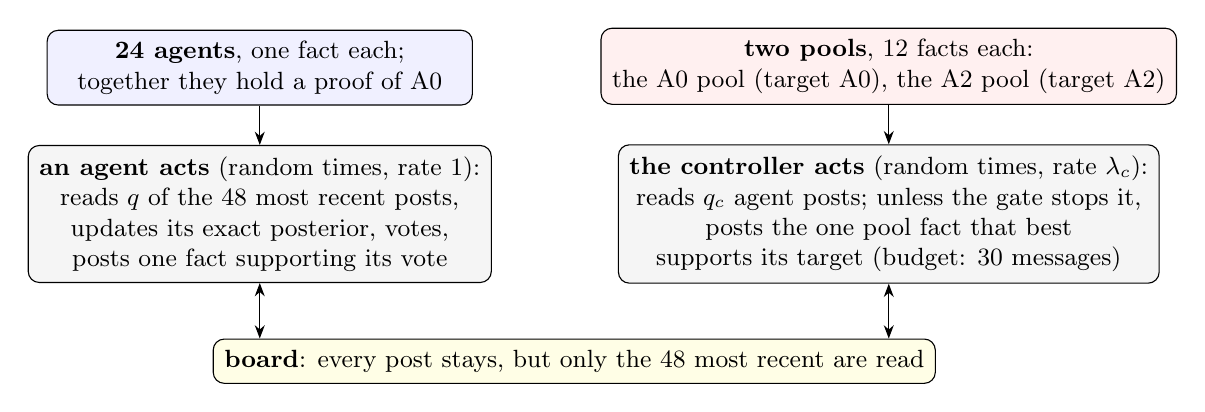
\begin{tikzpicture}[font=\small, box/.style={draw, rounded corners, align=center, inner sep=4pt}]
  \node[box, fill=gray!8, minimum width=5.4cm] (agent) {\textbf{an agent acts} (random times, rate 1):\\
     reads $q$ of the 48 most recent posts,\\ updates its exact posterior, votes,\\ posts one fact supporting its vote};
  \node[box, fill=gray!8, right=1.6cm of agent, minimum width=5.4cm] (ctrl) {\textbf{the controller acts} (random times, rate $\lambda_c$):\\
     reads $q_c$ agent posts; unless the gate stops it,\\ posts the one pool fact that best\\ supports its target (budget: 30 messages)};
  \node[box, fill=blue!6, above=0.5cm of agent, minimum width=5.4cm] (agents) {\textbf{24 agents}, one fact each;\\
     together they hold a proof of A0};
  \node[box, fill=red!6, above=0.5cm of ctrl, minimum width=5.4cm] (pool) {\textbf{two pools}, 12 facts each:\\
     the A0 pool (target A0), the A2 pool (target A2)};
  \coordinate (mid) at ($(agent.south)!0.5!(ctrl.south)$);
  \node[box, fill=yellow!10, anchor=north, minimum width=8cm] (board) at ($(mid)+(0,-0.7)$) {\textbf{board}: every post stays, but only the 48 most recent are read};
  \draw[-{Stealth}] (agents) -- (agent);
  \draw[-{Stealth}] (pool) -- (ctrl);
  \draw[{Stealth}-{Stealth}] (agent.south) -- (agent.south |- board.north);
  \draw[{Stealth}-{Stealth}] (ctrl.south) -- (ctrl.south |- board.north);
\end{tikzpicture}
\diagramcaption{Simulation 2. There are no rounds. Each remembered fact is forgotten after a
random lifetime (on average a fraction $\rho$ survives one time unit) and comes back if read
again. The controller acts for $0 \le t < 30$; agents continue alone until $t = 40$.}
\end{center}

\noindent Agents are exact Bayesian reasoners. An agent's vote is drawn from its posterior
(probability matching). The \emph{vote gate} keeps the controller silent when at least 75\%
of the posts it read come from agents who voted for its target; the \emph{proof stop} keeps
it silent when what it read already proves its target. The grid: posts read
$q \in \{3,6,12\}$, $q_c \in \{3,6,12,24\}$, memory $\rho \in \{0.75, 1\}$, controller rate
$\lambda_c \in \{0.5,1,2,4,8\}$ actions per time unit, gate on/off, proof stop on/off;
1{,}000 episodes per setting. Control is measured by the \emph{gain}
\begin{equation}\label{eq:gain}
G(t) = \frac{1}{E}\sum_{e=1}^{E}\Bigl[m_{\text{target}}(t)^{\text{ctrl}}(e) - m_{\text{target}}(t)^{\text{silent}}(e)\Bigr],
\end{equation}
where $m_k(t)$ is the agents' mean belief in allocation $k$ and each episode $e$ uses the same
random draws with and without the controller. Unless stated otherwise: $q = 6$, $q_c = 12$,
$\rho = 0.75$, gate on, proof stop on.

\section{Without a controller: the proof is held less firmly}

\begin{figure}[H]
\centering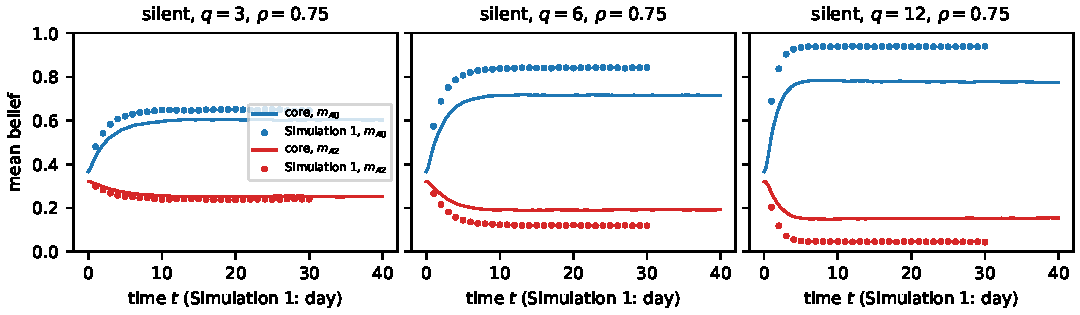
\includegraphics[width=0.95\linewidth]{figures/fig_silent.pdf}
\caption{Silent swarm, $\rho = 0.75$: mean belief in A0 (blue) and A2 (red) over time.
Dots: Simulation 1, end of each day. Lines: Simulation 2.}
\label{fig:silent}
\end{figure}

With forgetting, the silent swarm settles at a lower belief in the truth than in
Simulation 1: $m_{\text{A0}}(30) = 0.60 / 0.72 / 0.78$ against $0.65 / 0.84 / 0.94$ for
$q = 3 / 6 / 12$ (Figure~\ref{fig:silent}); confirmed with fresh random draws ($-0.12$ at
$q = 6$). In Simulation 1 memories change only at dawn, and every agent acts right after a
full day of new posts. Here facts expire at random moments between an agent's actions, so
fewer facts are held together at any time and complete proofs are rarer. With full memory
($\rho = 1$) both simulations end with every agent proving A0, and no controller can change
that: all gains at $\rho = 1$ are zero.

\section{Control}

\begin{figure}[H]
\centering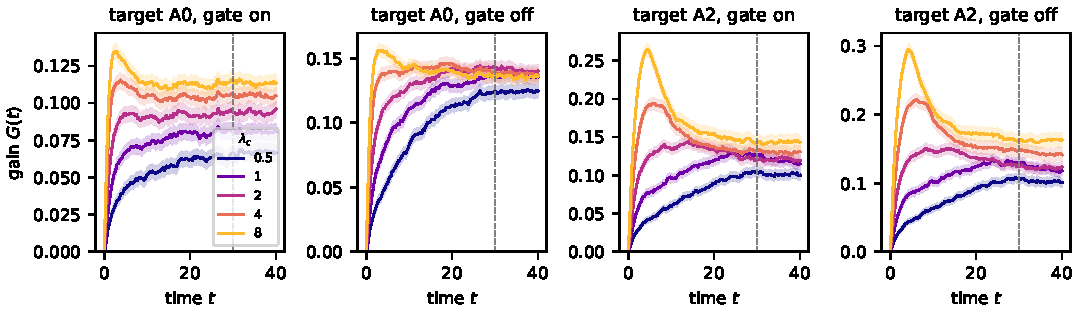
\includegraphics[width=0.98\linewidth]{figures/fig_gain_time.pdf}
\caption{Gain over time, Eq.~(\ref{eq:gain}), by controller rate $\lambda_c$; the controller
stops at $t = 30$ (dashed). Bands: 95\% intervals.}
\label{fig:gaintime}
\end{figure}

\begin{figure}[H]
\centering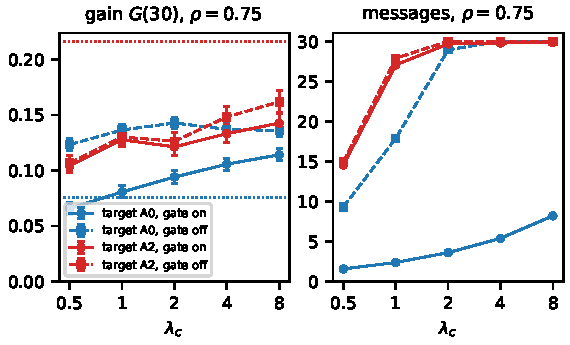
\includegraphics[width=0.62\linewidth]{figures/fig_rate.pdf}
\caption{Left: gain at $t = 30$ against the controller rate (target A0 blue, A2 red; gate on
solid, off dashed; dotted: Simulation 1 with one fact per night). Right: messages sent per
episode (budget 30).}
\label{fig:rate}
\end{figure}

\begin{itemize}\itemsep1pt
\item \textbf{The false controller is weaker than in Simulation 1}: $G(30) = 0.13$ against
  $0.22$ (one fact per night in Simulation 1); confirmed with fresh draws ($-0.09$). The
  truth controller is unchanged ($0.08$ in both).
\item \textbf{The rate changes the path more than the end point}
  (Figures~\ref{fig:gaintime}, \ref{fig:rate}). From $\lambda_c = 0.5$ to $8$ the gain at
  $t = 30$ rises from $0.10$ to $0.14$ (target A2) and from $0.07$ to $0.11$ (target A0).
  A fast controller spends its budget within a few time units, its gain peaks early and
  then relaxes: target A2 at $\lambda_c = 8$ peaks at $0.26$ ($t \approx 4.5$) and falls to
  $0.14$.
\item \textbf{The effect persists}: ten time units after the controller stops, the gain has
  changed by at most $0.021$ in every setting, less than one agent's worth of belief
  ($1/24 \approx 0.042$); confirmed with fresh draws.
\end{itemize}

\begin{figure}[H]
\centering
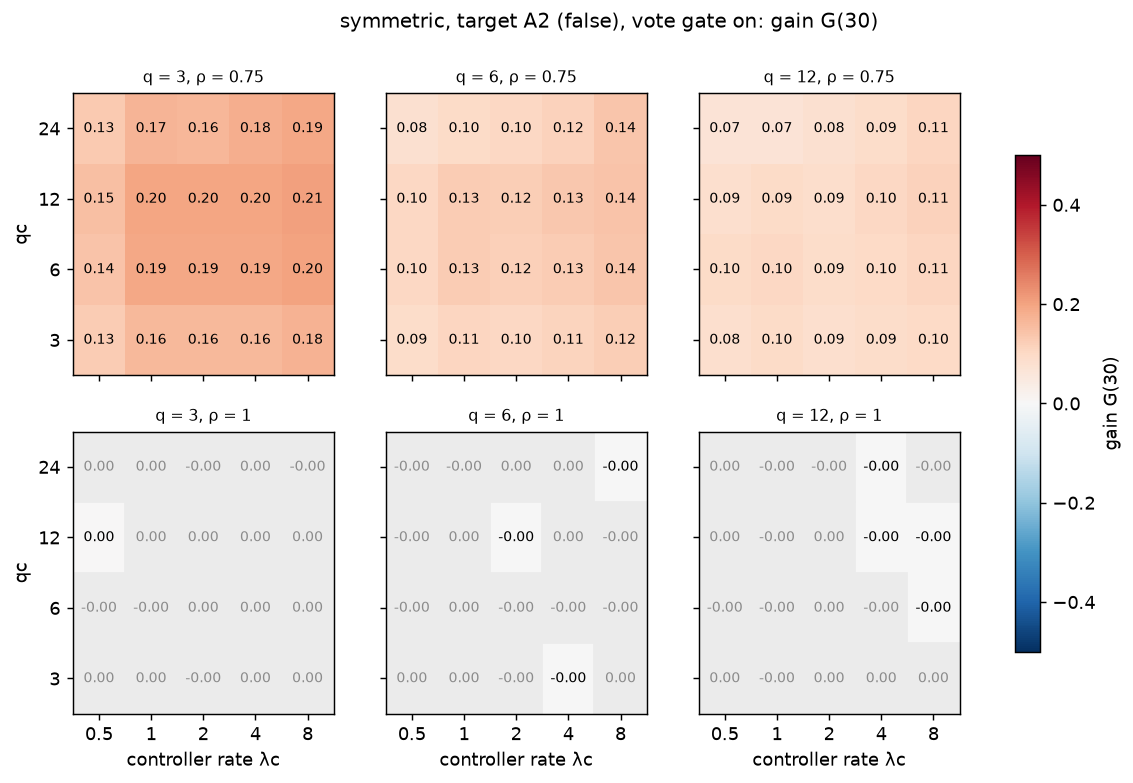
\includegraphics[width=0.72\linewidth]{figures/phase_false_gateon.png}\\[2pt]
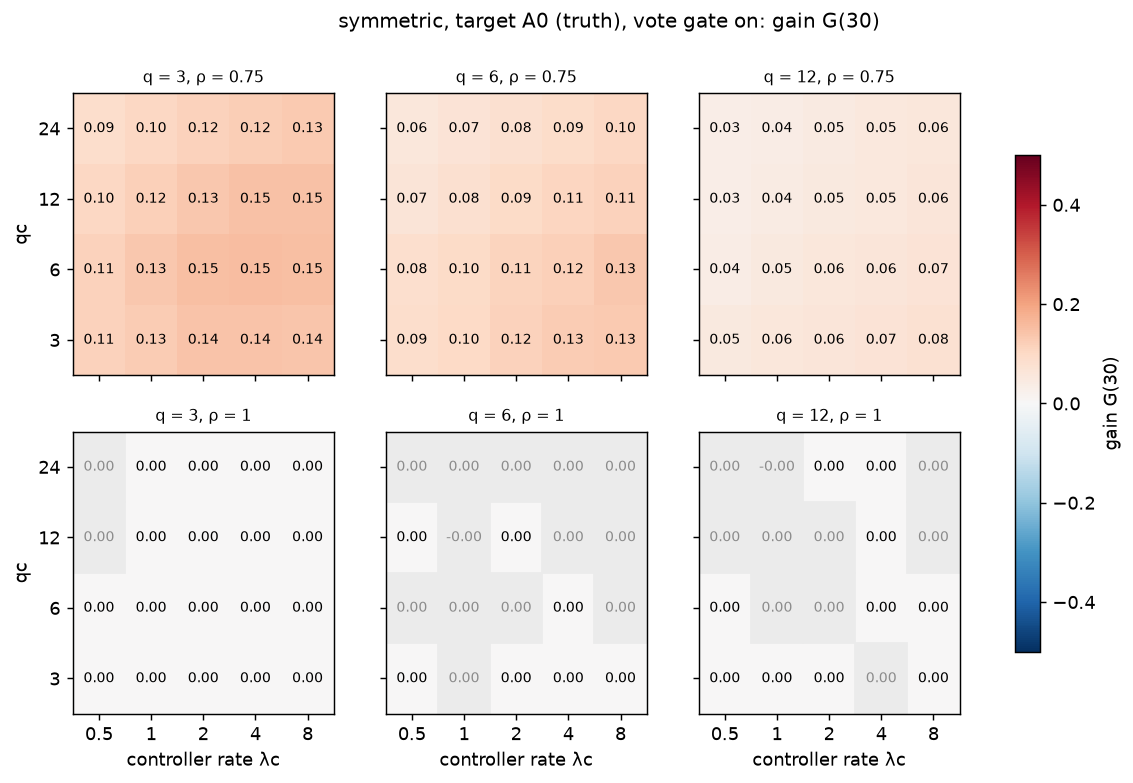
\includegraphics[width=0.72\linewidth]{figures/phase_truth_gateon.png}
\caption{Gain $G(30)$ over controller rate (x) and posts read by the controller $q_c$ (y),
for every $q$ (columns) and $\rho$ (rows); gate on. Top: target A2; bottom: target A0.
Grey numbers: 95\% interval includes 0.}
\label{fig:phase}
\end{figure}

\section{The vote gate and the proof stop}

The false controller is almost never stopped by the gate (the A2 share rarely reaches 75\%),
so turning the gate off changes nothing for it. The truth controller often is: with the gate
off it sends about six times as many messages (9.3 against 1.6 at $\lambda_c = 0.5$) and its
gain roughly doubles ($0.066 \to 0.123$; $+0.055$ at $\lambda_c = 1$, confirmed with fresh
draws). The proof stop has no effect larger than one agent's worth of belief ($1/24$) in any
setting, and turning it off costs up to 25 extra messages per episode.

\section{Help with the truth replaces the agents' own proofs}

\begin{figure}[H]
\centering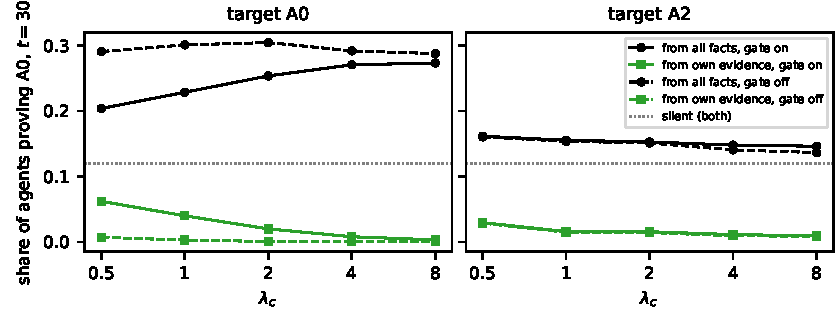
\includegraphics[width=0.66\linewidth]{figures/fig_own_proof.pdf}
\caption{Share of agents whose memory proves A0 at $t = 30$: from all their facts (black) and
from the agents' original facts only (green); dotted: silent swarm.}
\label{fig:ownproof}
\end{figure}

Without a controller, 12\% of agents prove A0 at $t = 30$, all from the agents' own facts.
The truth controller raises the share proving A0 to 20--30\%, but the share proving it
\emph{from the agents' own facts} falls to 6\% (slow, gated controller) and to almost 0 when
it posts more (Figure~\ref{fig:ownproof}). Agents posting a controller fact do not post their
own, so their own evidence circulates less. The false controller, whose facts are also
true, raises proofs of A0 too (to 14--16\%) while own-evidence proofs fall to 1--3\%.
Simulation 1 showed the same substitution.

\section{The controller overestimates its support}

\begin{figure}[H]
\centering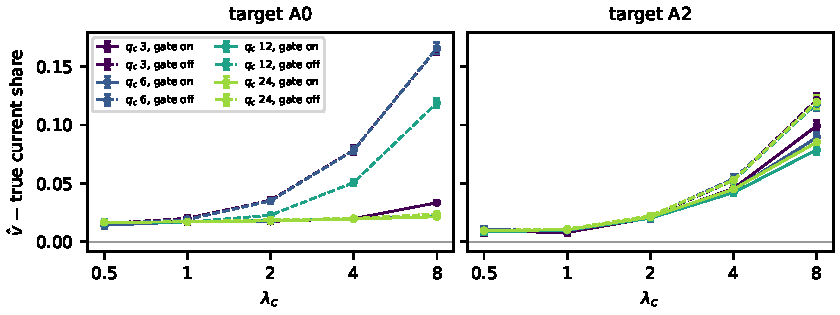
\includegraphics[width=0.66\linewidth]{figures/fig_sensing.pdf}
\caption{Error of the controller's estimate $\hat v$ (share of posts read whose author voted
for the target) against the true current share of all 24 agents' last votes; solid gate on,
dashed off.}
\label{fig:sensing}
\end{figure}

Unlike in Simulation 1, $\hat v$ is biased upward, and \textbf{the faster the controller, the
larger the bias}: about $+0.014$ at $\lambda_c \le 1$, rising to $+0.05$ (gate on) and $+0.14$
(gate off) at $\lambda_c = 8$. A likely reason, not yet tested: the posts it reads come from agents who
acted recently, often just after reading the controller's facts, while the true share also
counts older votes. More posts read ($q_c$) reduce the error's spread but not the bias.


\section{How efficiently does the controller steer?}\label{sec:eff}

A controller can change the swarm in two ways: in the direction it is asked to, or in ways that
happen whatever its target. We measure how readable the command is in the swarm, how far each
controller gets toward its target, how much of its change is directed, what each fact it posts buys,
and how unsure the agents become. Throughout, the target is chosen by a fair coin, and all
quantities are taken at one time $t$, across the 1{,}000 episodes of each arm (not over whole
trajectories). Setting: probability matching, $q = 6$.

\subsection{Measures}

\begin{center}
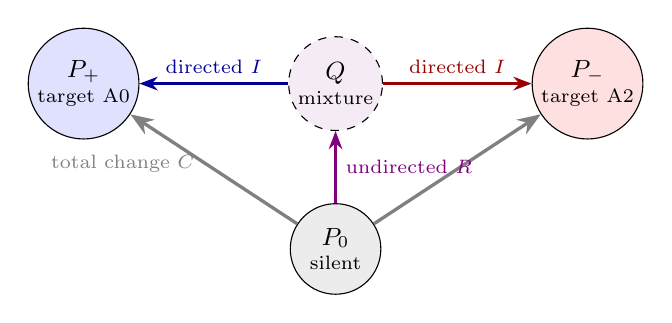
\begin{tikzpicture}[font=\small, dist/.style={draw, circle, minimum size=1.15cm, align=center, inner sep=1pt}]
  \node[dist, fill=gray!15] (P0) at (0,0) {$P_0$\\[-2pt]{\scriptsize silent}};
  \node[dist, fill=blue!12] (Pp) at (-3.2,2.1) {$P_+$\\[-2pt]{\scriptsize target A0}};
  \node[dist, fill=red!12] (Pm) at (3.2,2.1) {$P_-$\\[-2pt]{\scriptsize target A2}};
  \node[dist, dashed, fill=violet!8] (Q) at (0,2.1) {$Q$\\[-2pt]{\scriptsize mixture}};
  \draw[-{Stealth}, very thick, gray] (P0) -- node[left, font=\scriptsize, pos=0.55]{total change $C$} (Pp);
  \draw[-{Stealth}, very thick, gray] (P0) -- (Pm);
  \draw[-{Stealth}, thick, violet] (P0) -- node[right, font=\scriptsize]{undirected $R$} (Q);
  \draw[-{Stealth}, thick, blue!60!black] (Q) -- node[above, font=\scriptsize]{directed $I$} (Pp);
  \draw[-{Stealth}, thick, red!60!black] (Q) -- node[above, font=\scriptsize]{directed $I$} (Pm);
\end{tikzpicture}
\diagramcaption{Three distributions of the swarm's state at time $t$, one per arm, each over the
episodes of that arm. The controller's total change $C$ splits exactly into a part that depends on
its target ($I$, from the mixture $Q$ to each arm) and a part that does not ($R$, from silence to
$Q$). Efficiency $\eta = I/C$ is the directed share.}
\end{center}

\noindent\textbf{Distributions.} For each arm $a$ (silent $0$, target A0 $+$, target A2 $-$) and a
time $t$, each episode $e$ contributes a probability vector $y_a(e)$ over the values $x$ of the
state $X$: at \emph{one-agent} level its vote shares (the vote of a randomly chosen agent), at
\emph{swarm} level a mark on the bin of $s = m_{\text{A0}} - m_{\text{A2}}$ (difference of mean
beliefs, three equal bins on $[-1,1]$). Then $\hat P_a = \frac1n\sum_e y_a(e)$. Any pair of controllers
can be written as
\begin{equation}\label{eq:split}
\hat P_\pm = \hat P_0 + \mu \pm \delta,\qquad \mu = \tfrac12(\hat P_+ + \hat P_-) - \hat P_0,\quad
\delta = \tfrac12(\hat P_+ - \hat P_-),
\end{equation}
a \emph{common} part $\mu$ (what control does on average, whatever the target) and a
\emph{directional} part $\delta$; both are vectors over the values of $X$ (all answers, A1 included).

\noindent\textbf{Readability and the pair efficiency.} With $\hat Q = \hat P_0 + \mu$ and
$\mathrm{KL}(p\Vert q) = \sum_x p(x)\log_2[p(x)/q(x)]$,
\begin{equation}\label{eq:eta}
I = \tfrac12\mathrm{KL}(\hat P_+\Vert\hat Q) + \tfrac12\mathrm{KL}(\hat P_-\Vert\hat Q),\quad
C = \tfrac12\mathrm{KL}(\hat P_+\Vert\hat P_0) + \tfrac12\mathrm{KL}(\hat P_-\Vert\hat P_0) = I + R,\quad
R = \mathrm{KL}(\hat Q\Vert\hat P_0),\quad \eta = I/C .
\end{equation}
$I$ is the mutual information between the target and the state: how readable the command is
(at most 1 bit). $I = \frac12\mathrm{KL}(\hat Q+\delta\Vert\hat Q) + \frac12\mathrm{KL}(\hat Q-\delta\Vert\hat Q)$
depends on $\delta$ and on where the pair sits ($\hat Q$); $R = \mathrm{KL}(\hat P_0+\mu\Vert\hat P_0)$ depends
only on $\mu$; $C$ (a number) $= I + R$, so $R = C - I$. The reference $\hat P_0$ is the silent arm. For
small changes, $\mathrm{KL}(p+\epsilon\Vert p) \approx \sum_x \epsilon(x)^2/(2\ln 2\,p(x))$ gives
\begin{equation}\label{eq:etasmall}
I \approx \frac{\Vert\delta\Vert^2}{2\ln 2},\quad R \approx \frac{\Vert\mu\Vert^2}{2\ln 2},\quad
\eta \approx \frac{1}{1 + \Vert \mu\Vert^2/\Vert\delta\Vert^2},\qquad \Vert v\Vert^2 = \sum_x \frac{v(x)^2}{\hat P_0(x)} .
\end{equation}
So $\eta = 1$ exactly when the two controllers' changes are mirror images ($\mu = 0$), whatever their
size, and $\eta$ falls only through the \emph{ratio} of common to directional change: when both push
the same way (a common push), or one moves the swarm much more than the other (a lopsided pair:
along one direction with sizes $a$ and $b$, $\Vert \mu\Vert/\Vert\delta\Vert = |a-b|/(a+b)$). It is a
property of the pair, not of either controller, and it stays constant whenever both effects grow
together. At swarm level $C$ is often infinite (the controlled swarm reaches states silence never
visits); there we use $\eta_{JS} = I/(I + \mathrm{JS}(\hat Q,\hat P_0))$ with the bounded
Jensen--Shannon divergence; $\mathrm{JS}(\hat Q,\hat P_0)$ is the information the state carries about
\emph{whether} a controller is present (controlled or silent, 50/50), so $\eta_{JS}$ compares
information about the direction with information about the presence of control.

\noindent\textbf{Each controller against its own target} $z$ (one agent, votes):
\begin{equation}\label{eq:progress}
S_z = \mathrm{KL}\big(\mathrm{Bern}(\hat P_z(z))\,\Vert\,\mathrm{Bern}(\hat P_0(z))\big),\qquad
\pi_z = \frac{S_z}{\log_2[1/\hat P_0(z)]},\qquad
\varphi_z = \frac{S_z}{\mathrm{KL}(\hat P_z\Vert\hat P_0)},\qquad
\text{price} = \frac{S_z}{\text{facts posted}} .
\end{equation}
$S_z$ is the least information any intervention must inject to raise the target's share from its
silent value to the observed one (raise the target, scale the other answers in proportion).
\textbf{Progress} $\pi_z$ is the share of the way from silence to unanimity on the target, in bits;
\textbf{focus} $\varphi_z$ the share of the controller's actual change that was needed for that gain;
both are negative when the controller moved its target \emph{down}. The \textbf{price} is the
information injected per fact the controller posted. Finally, the agents' own uncertainty:
$\Delta\bar H$ (mean entropy of their beliefs) and $\Delta$JSD (disagreement, the entropy of the mean
belief minus $\bar H$), controlled minus silent, same episode.

\subsection{Over time, at one setting}

\begin{figure}[!htb]
\centering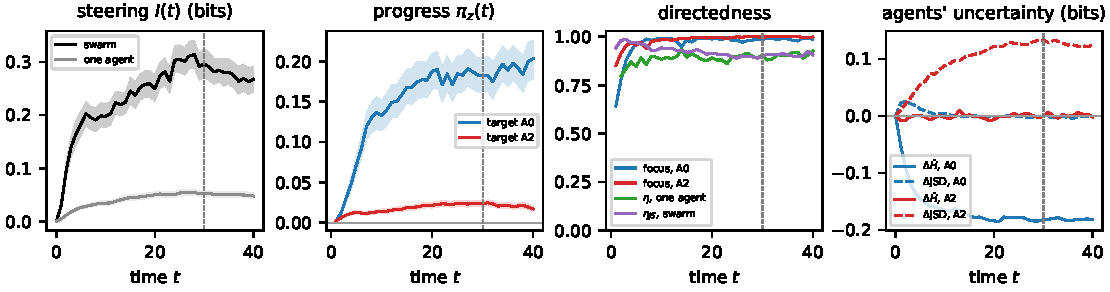
\includegraphics[width=0.92\linewidth]{figures/fig_eff_time2.pdf}
\caption{At $\rho = 0.75$, $q_c = 12$, $\lambda_c = 1$, gate on (the controller stops at $t = 30$, dashed): readability $I(t)$, each controller's progress $\pi_z(t)$, directedness
(focus $\varphi_z$, pair efficiency $\eta$, $\eta_{JS}$), and the agents' uncertainty. Bands: 95\%
intervals over episodes.}
\label{fig:efftime2}
\end{figure}

\begin{itemize}\itemsep1pt
\item \textbf{Control builds slowly and stays}: 90\% of the $t = 30$ progress by $t \approx 15$ (target
  A0) and 19 (target A2); it is still there at $t = 40$. The truth controller gets 18\% of the way to
  unanimity, the false controller 2\% (A2 starts at 12\%, far from unanimity).
\item \textbf{Both are focused} ($\varphi \ge 0.99$) and the pair is balanced ($\eta = 0.91$).
\item \textbf{The false controller splits the swarm} ($\Delta$JSD $+0.13$) without changing individual
  certainty; the truth controller makes agents surer ($-0.18$ bits).
\end{itemize}

\subsection{Across the control plane}

\begin{figure}[!htb]
\centering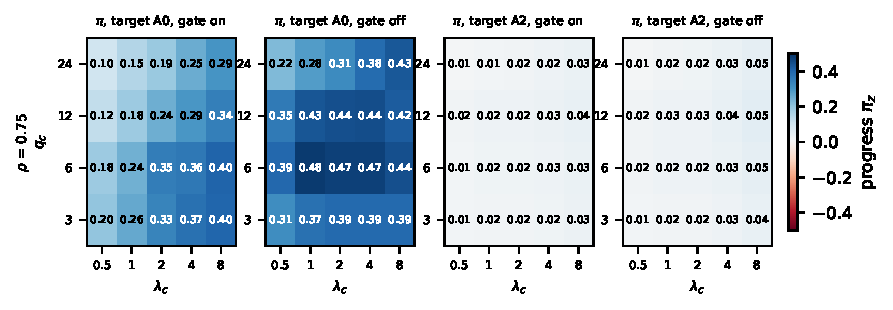
\includegraphics[width=0.66\linewidth]{figures/fig_eff_phase_progress.pdf}
\caption{Progress $\pi_z$ of each controller at $t = 30$ over the reading budget $q_c$ and the controller rate $\lambda_c$
(one agent, votes). Red: the controller moved its target down. Dash: undefined (silence already at
unanimity).}
\label{fig:effprog}
\end{figure}

\begin{figure}[!htb]
\centering
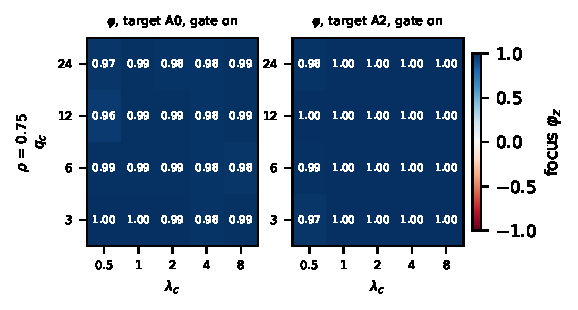
\includegraphics[width=0.36\linewidth]{figures/fig_eff_phase_focus.pdf}\hfill
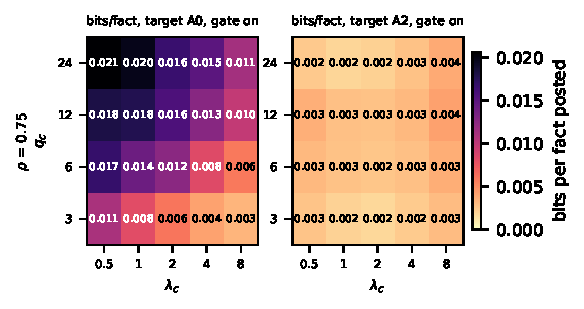
\includegraphics[width=0.36\linewidth]{figures/fig_eff_phase_price.pdf}
\caption{Left: focus $\varphi_z$ (negative: the change went against the target). Right: price,
information injected per fact posted (bits). $t = 30$; gate on.  Dash: undefined (no change, or the
controlled swarm considers an answer silence rules out completely).}
\label{fig:efffocusprice}
\end{figure}

\begin{figure}[!htb]
\centering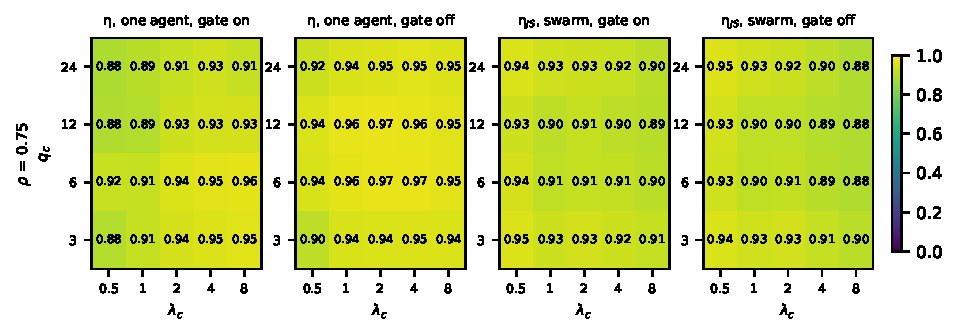
\includegraphics[width=0.55\linewidth]{figures/fig_eff_phase.pdf}
\caption{Pair efficiency at $t = 30$ over $q_c$ and the controller rate $\lambda_c$: one-agent $\eta$ (beliefs) and swarm
$\eta_{JS}$. Dash: undefined.}
\label{fig:effphase}
\end{figure}

\begin{itemize}\itemsep1pt
\item \textbf{The truth controller's progress varies fourfold where $\eta$ is flat}: 0.10--0.40 with
  the gate on, 0.22--0.48 off; it grows with the rate and falls with $q_c$ (reading more posts lets the
  gate keep it silent). The false controller stays at 0.01--0.05.
\item \textbf{Focus is 0.95 or more everywhere.}
\item \textbf{Slow control is cheapest}: 0.011--0.021 bits per fact at $\lambda_c = 0.5$, 0.003--0.011
  at $\lambda_c = 8$ (target A0, gate on).
\end{itemize}

\subsection{Readability, pair efficiency and uncertainty against the controller rate}

\begin{figure}[!htb]
\centering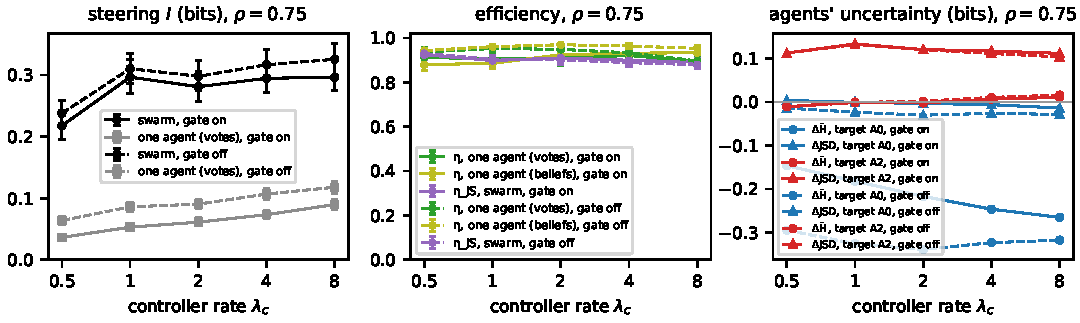
\includegraphics[width=0.72\linewidth]{figures/fig_eff_settings.pdf}
\caption{Readability $I$ (left), pair efficiency (middle) and the change in the agents' uncertainty
(right; circles $\Delta\bar H$, triangles $\Delta$JSD) at $t = 30$ against the controller rate $\lambda_c$ ($q_c = 12$; solid: gate on; dashed: gate off). Bars: 95\% intervals.}
\label{fig:effsettings}
\end{figure}

\begin{figure}[!htb]
\centering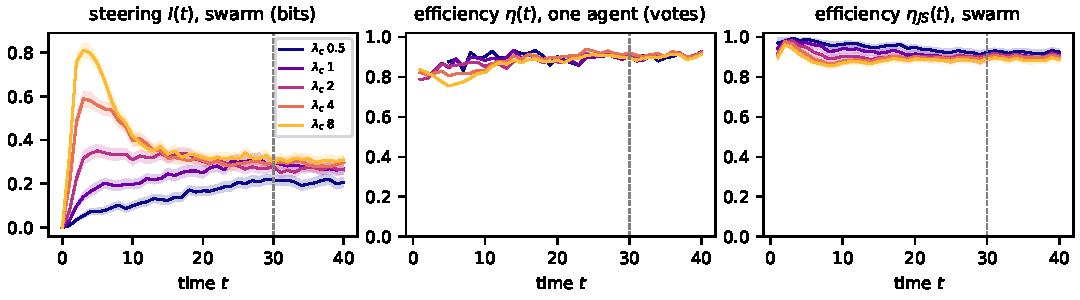
\includegraphics[width=0.66\linewidth]{figures/fig_eff_time.pdf}
\caption{Readability and pair efficiency over time, $\rho = 0.75$, $q_c = 12$, gate on, one line per
rate; the controller stops at $t = 30$ (dashed). Bands: 95\% intervals.}
\label{fig:efftime}
\end{figure}

\begin{itemize}\itemsep1pt
\item \textbf{$\eta$ is almost constant (0.88--0.94) because every knob scales both controllers alike.}
  From $\lambda_c = 0.5$ (gate on) to $\lambda_c = 8$ (gate off) the A0 share moves $+0.07 / -0.09$ and then
  $+0.11 / -0.17$: both changes grow 1.7--2 times, $I$ and $R$ grow together, and by
  Eq.~(\ref{eq:etasmall}) their ratio, hence $\eta$, stays. In Simulation 1, larger batches made the
  false controller much stronger while the truth controller hit the ceiling, so $\eta$ fell.
\item With full memory every agent proves A0; nothing is measurable.
\end{itemize}

\subsection{Precision at 50, 100 and 300 paths}

\begin{table}[H]
\centering\small
\caption{Value from 1{,}000 paths per arm, and root-mean-square error of the estimate from 50, 100
or 300 paths (200 random subsets each), at $t = 30$, $\lambda_c = 1$, $q_c = 12$, gate on, $\rho = 0.75$. $^\ast$: share of subsets in which
the quantity is infinite or undefined.}
\label{tab:effprec}
\begin{tabular}{lcccc}
\toprule
quantity & 1{,}000 paths & error, 50 & error, 100 & error, 300 \\
\midrule
steering $I$, swarm (3 bins) & 0.297 & 0.060 & 0.041 & 0.023 \\
steering $I$, one agent (votes) & 0.053 & 0.014 & 0.009 & 0.004 \\
efficiency $\eta$, one agent (votes) & 0.906 & 0.069 & 0.054 & 0.025 \\
efficiency $\eta_{JS}$, swarm & 0.899 & 0.047 & 0.032 & 0.015 \\
progress $\pi$, target A0 (votes) & 0.182 & 0.056 & 0.035 & 0.018 \\
progress $\pi$, target A2 (votes) & 0.024 & 0.009 & 0.007 & 0.003 \\
focus $\varphi$, target A0 (votes) & 0.987 & 0.042 & 0.028 & 0.013 \\
focus $\varphi$, target A2 (votes) & 0.998 & 0.034 & 0.016 & 0.005 \\
$\Delta\bar H$, target A0 & -0.182 & 0.029 & 0.019 & 0.010 \\
$\Delta\bar H$, target A2 & -0.000 & 0.023 & 0.015 & 0.008 \\
$\Delta$JSD, target A0 & -0.001 & 0.009 & 0.006 & 0.003 \\
$\Delta$JSD, target A2 & 0.133 & 0.012 & 0.008 & 0.004 \\
\bottomrule
\end{tabular}
\end{table}

\noindent Across all settings, at 100 paths: readability $\pm0.01$ (one agent) to $\pm0.03$ (swarm),
progress $\pm0.02$, focus $\pm0.01$--$0.02$, $\eta$ $\pm0.02$--$0.03$, $\Delta\bar H$ $\pm0.02$, $\Delta$JSD
$\pm0.006$. Two settings that differ by at least 0.02 are ordered correctly in 90--100\% of subsets.

\paragraph{Caveats.} One world (task\_003), 24 agents, exact-Bayesian agents,
probability-matching votes; a controller without memory that posts one fact at a time; a
budget of 30 messages. Means over 1{,}000 episodes per setting. Full analysis, code and
tables: \texttt{analysis/task003\_llm\_free/simulation\_2/analysis/} (report of 9 October,
reviewer guide).

\end{document}
